\documentclass[t]{beamer} %t=points top alligned

\usetheme{PaloAlto} %names of cities, and color is names of animals
\usepackage{caption}
\captionsetup[figure]{labelformat=empty}% redefines the caption setup of the figures environment in the beamer class.

\usebeamercolor{Green}
\usepackage{lipsum}
\usepackage{array}
\newcolumntype{L}{>{\centering\arraybackslash}m{1.8cm}}

\newcommand\blfootnote[1]{%
	\begingroup
	\renewcommand\thefootnote{}\footnote{#1}%
	\addtocounter{footnote}{-1}%
	\endgroup
}
\logo{\includegraphics[scale=0.035]{logo}}
%adobe reader >11 for sound and animation
%nairsujath@gmail.com
\title{Development of Low Power Wireless Sensor Network using Zigbee Protocol for Terrace Farm}
\subtitle
{	EE 692 R \& D
}
\author
{	
	Saurav Shandilya (153076004) \\
	M.Tech (Electronic Systems)\\
	Department of Electrical Engineering \\
	Supervisor: Dr. Kavi Arya
}

\date{} %for not inserting date automatically

%***************** Packages for Graphics & Figures *******************%
\usepackage{graphicx} %%For loading image files
\graphicspath{ {images/} } %folder-location for images

\usepackage{amsmath}

\begin{document}
\setbeamertemplate{sidebar left}{}
\maketitle
\begin{frame}{Agenda}
\tableofcontents
\end{frame}

\section{Introduction}
\begin{frame}{Introduction}
\begin{itemize}
\item \large{Why do we want WSN on Terrace Farm? }
	\begin{itemize}
	\item Automatic irrigation
    \item Crop health monitoring - Leaf wetness sensor, soil temperature
    \item Measurement of light intensity and pH levels
    \item Terrace farm as prototype/testbed to test solution at small level \\[0.5cm]
	\end{itemize}	
\item \large{Why and how much low power?}
	\begin{itemize}
	\item Typically a battery operated on 2AA or rechargeable battery should last for months if not years.
    \item Optimal hardware choice and software design based on application
	\end{itemize}
	
\end{itemize}
\end{frame}

\begin{frame}{Wireless Protocols}
\begin{table}[!h]
	%\renewcommand{\arraystretch}{1.5} %specific row width
	\caption{Comparision of Bluetooth, Zigbee and Wifi }
	\label{Effect of data sampling frequency on Disaggregration}
	\centering
	\begin{tabular}{|L|L|L|L|}
		\hline
		& Bluetooth & Zigbee & Wi-Fi \\
        \hline
        IEEE Specs & 802.15.1 & 802.15.4 & 802.11 \\
        \hline
        Frequency Band & 2.4GHz & 868/915 MHz or 2.4 GHz  & 2.4 GHz; 5GHz\\        
        \hline
        Signal Rate & 1Mb/s & 250Kb/s & 54Mb/s \\
        \hline
        Range & 10m & 10-100m & 100m \\
        \hline
        $T_x$ Current (mA) & 57 & 24.7 & 219 \\
        \hline
        $R_x$ Current (mA) & 47 & 27 & 215 \\
        \hline
	\end{tabular}
\end{table}

\end{frame}

\section{Low Power Design Consideration}
\begin{frame}{Computation of system power}
Average power consumption of a system can be expressed by equation \ref{equ:avg_power}:
\begin{equation}
	P_{avg} = (P_{active} + P_{sleep} + P_{transition})/T_{total}
    \label{equ:avg_power}
\end{equation}	
where: \\[0.5cm]
	$P_{active}$ = Power being consumed in active mode * Time for which system is active \\
    $P_{sleep}$ = Power being consumed in sleep mode * Time for which system is sleep \\
    $P_{transition}$ = Power consumed while making transition from sleep mode to active mode \\

\end{frame}

\begin{frame}{Power consumption of microcontroller}
The power consumption by CMOS circuit is given by equation \cite{sanam_MTP report}:
\begin{equation}
	 P = f*C_L*V_{dd}^2
     \label{equ:cmos_power}
\end{equation}

Where: \\
	$P$: Power Consumed 
    
    $f$: Operating Frequency of controller
    
    $C_L$: Load capacitance
    
    $V_{dd}$: Supply Voltage used to run the controller \\[0.5cm]
    
\begin{itemize}
\item Load capacitance $C_L$ is determined during IC design
\item Operating Frequency($f$) and Supply Voltage $V_{dd}$ can be controlled
\end{itemize}
\end{frame}

\begin{frame}{Low power design consideration }
\begin{itemize}
\item Pull all GPIO pins of microcontroller to low level to prevent leakage current \\ [0.5cm]
\item Selecting lowest possible operating voltage and frequencies to reduce current consumption \\[0.5cm]
\item Selecting proper low power mode \\[0.5cm]
\item Turn off peripherals when not used
\end{itemize}
\end{frame}

\section{Hardware Design}
\begin{frame}{Hardware Design - MSP430F5529}
\fboxsep=0pt
\noindent
\begin{minipage}[t]{0.48\linewidth}
\vspace{1cm}
\begin{figure}[!ht]
	\centering
\includegraphics[scale=0.2]{MSP430_launchpad}
\caption{\tiny image courtesy: \url{http://processors.wiki.ti.com}}
\label{fig:msp430_launchpad}
\end{figure}
\end{minipage}
\hfill
\begin{minipage}[t]{0.48\linewidth}
\begin{itemize}
\item Operating Voltage: 3.6V - 1.8V
\item 5 different clock source
\item Operating frequency: 10KHz - 25MHz
\item 3 clock signals
\item 12-bit ADC
\item 2 UART 
\item 63 IO pins
\end{itemize}
\end{minipage}

\end{frame}

\begin{frame}{Hardware Design - Xbee S2C}
\fboxsep=0pt
\noindent
\begin{minipage}[t]{0.48\linewidth}
\begin{figure}[!ht]
	\centering
\includegraphics[scale=0.3]{XBee}
\caption{\tiny image courtesy: \url{http://digi.com}}
\label{fig:xbee S2C}
\end{figure}
\end{minipage}
\hfill
\begin{minipage}[t]{0.48\linewidth}
\begin{itemize}
\item Operating Voltage: 2.1-3.6V
\item Indoor range: 60m
\item Outdoor range(LoS): 1200m
\item $T_x$ current: 45mA@3.3V
\item $R_x$ current: 31mA@3.3V
\item Sleep current: 1$\mu A$ 
\item Interface: UART/SPI
\end{itemize}
\end{minipage}
\end{frame}

\begin{frame}{Hardware Design - DHT22 Sensor}
\fboxsep=0pt
\noindent
\begin{minipage}[t]{0.48\linewidth}
\begin{figure}[!ht]
	\centering
\includegraphics[scale=0.3]{DHT22}
\caption{\tiny image courtesy: \url{http://sparkfun.com}}
\label{fig:dht22}
\end{figure}
\end{minipage}
\hfill
\begin{minipage}[t]{0.48\linewidth}
\begin{itemize}
\item Operating Voltage: 3.3-6V
\item Output signal: digital signal on Single wire 
\item Temp. Range: -40-80$ºC$
\item Humidity Range: 0-100\% RH
\item Resolution: 0.1
\item Sensing period: 2S
\item Active Current: 1mA
\item Sleep Current: 50$\mu$A
\end{itemize}
\end{minipage}
\end{frame}

\section{System Architecture}
\begin{frame}{System Architecture}

\begin{figure}[!ht]
	\centering
\includegraphics[scale=0.35]{sys_archi}
%\caption{Architecture of Wireless sensor network}
\label{fig:sys_archi}
\end{figure}

\end{frame}

\begin{frame}{Network Topologies}
\begin{figure}[!ht]
	\centering
\includegraphics[scale=0.4]{xbee_topologies}
\caption{\tiny image courtesy: \url{http://freemindscafe.com}}
\label{fig:topology}
\end{figure}
\end{frame}

\begin{frame}{Circuit Design - Schematic}
	\begin{figure}[!ht]
	\centering
\includegraphics[scale=0.6]{Stack_schematic_1}
\caption{Schematic for Stack}
%\label{fig:stack-schematic}
\end{figure}
\end{frame}

\begin{frame}{Circuit Design - PCB}
\fboxsep=0pt
\noindent
\begin{minipage}[t]{0.48\linewidth}
\vspace{2cm}
	\begin{figure}[!ht]
	\centering
\includegraphics[scale=0.6]{Stack_board}
%\caption{Schematic for Stack}
%\label{fig:stack-schematic}
	\end{figure}
\end{minipage}
\hfill
\begin{minipage}[t]{0.48\linewidth}
    \begin{figure}[!ht]
    \vspace{1.5cm}
	\centering
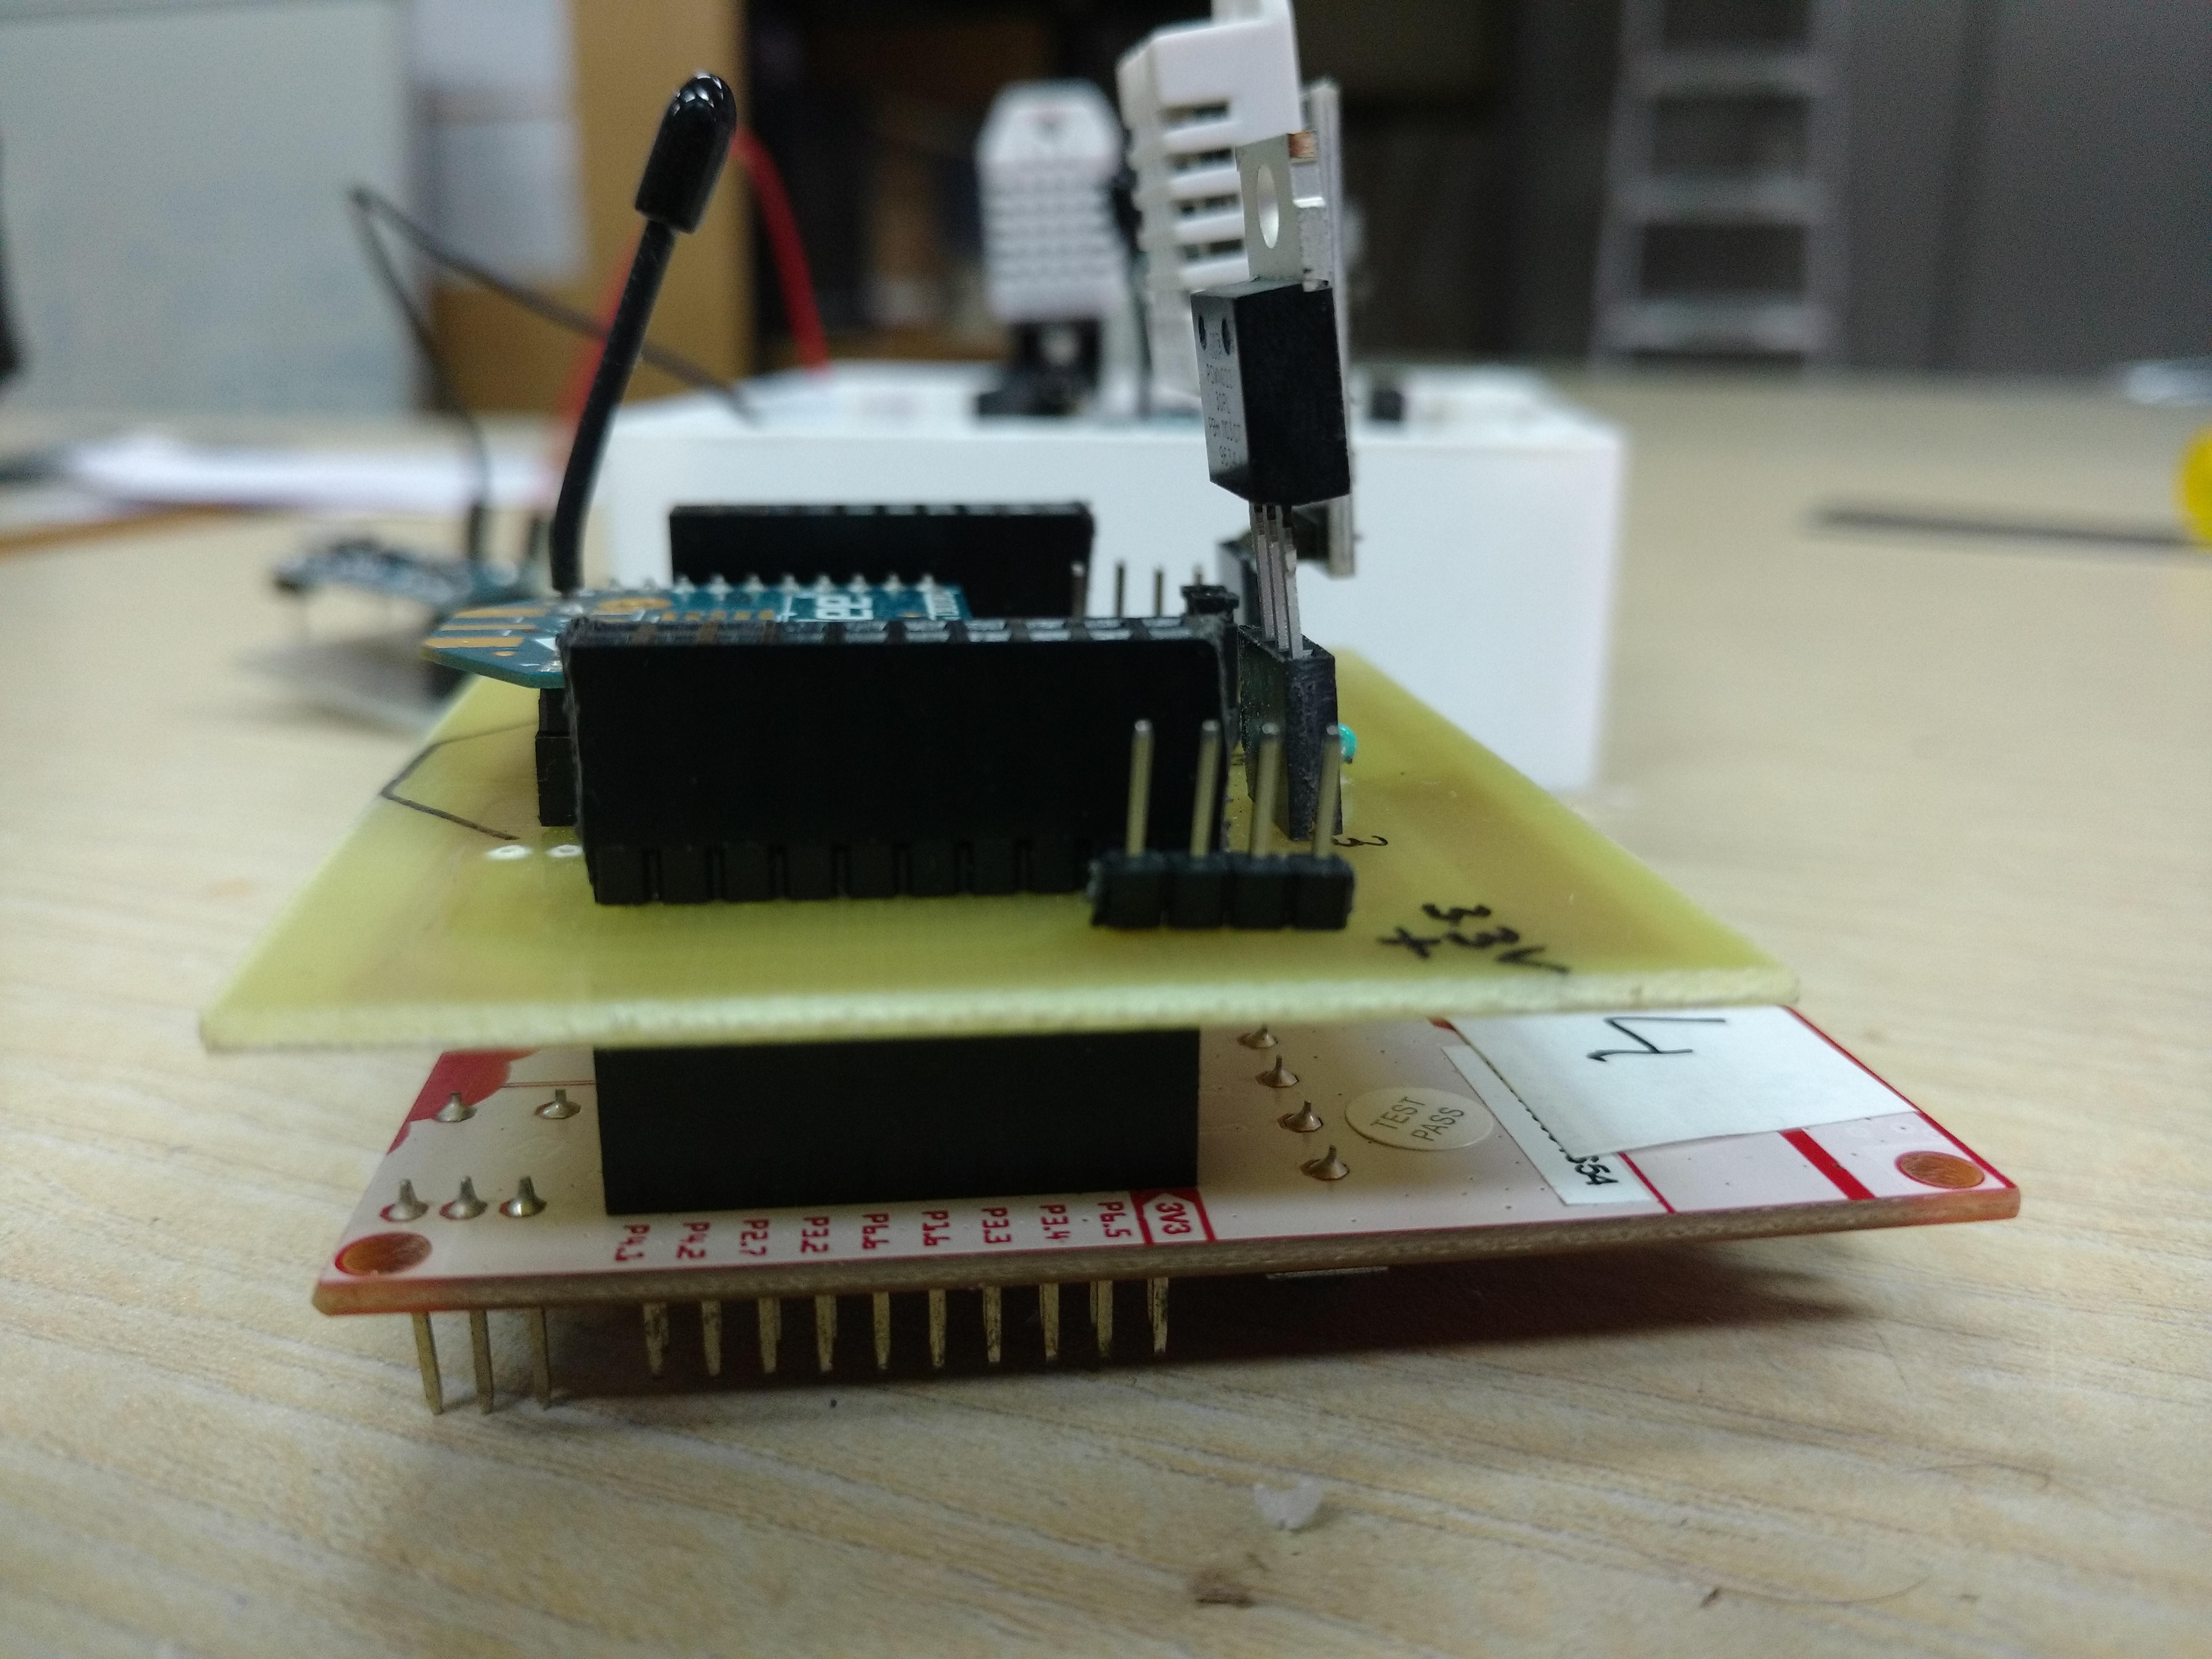
\includegraphics[scale=0.03]{stack}
%\caption{Stack}
%\label{fig:stack-schematic}
	\end{figure}
\end{minipage}
\end{frame} 

\section{Result}
\begin{frame}{Current Measurement for peripherals}
\begin{table}[!h]
	%\renewcommand{\arraystretch}{1.5} %specific row width
	\caption{Comparision of Bluetooth, Zigbee and Wifi }
	\label{Effect of data sampling frequency on Disaggregration}
	\centering
	\begin{tabular}{|L|L|L|}
		\hline
		Case & Current & Expected\\
        \hline
        No peripherals connected & 6$\mu$A & 2$\mu$A \\
        \hline
        DHT on & 1mA & 1mA \\        
        \hline
        DHT off & 18$\mu$A & 7$\mu$A \\
        \hline
        Xbee $R_x$ & 45mA & 31mA \\
        \hline
        xbee $T_x$ & 53mA & 45mA \\
        \hline
        
	\end{tabular}
\end{table}


\end{frame}

\begin{frame}{Current Measurement for peripherals}

\begin{figure}[!ht]
	\centering
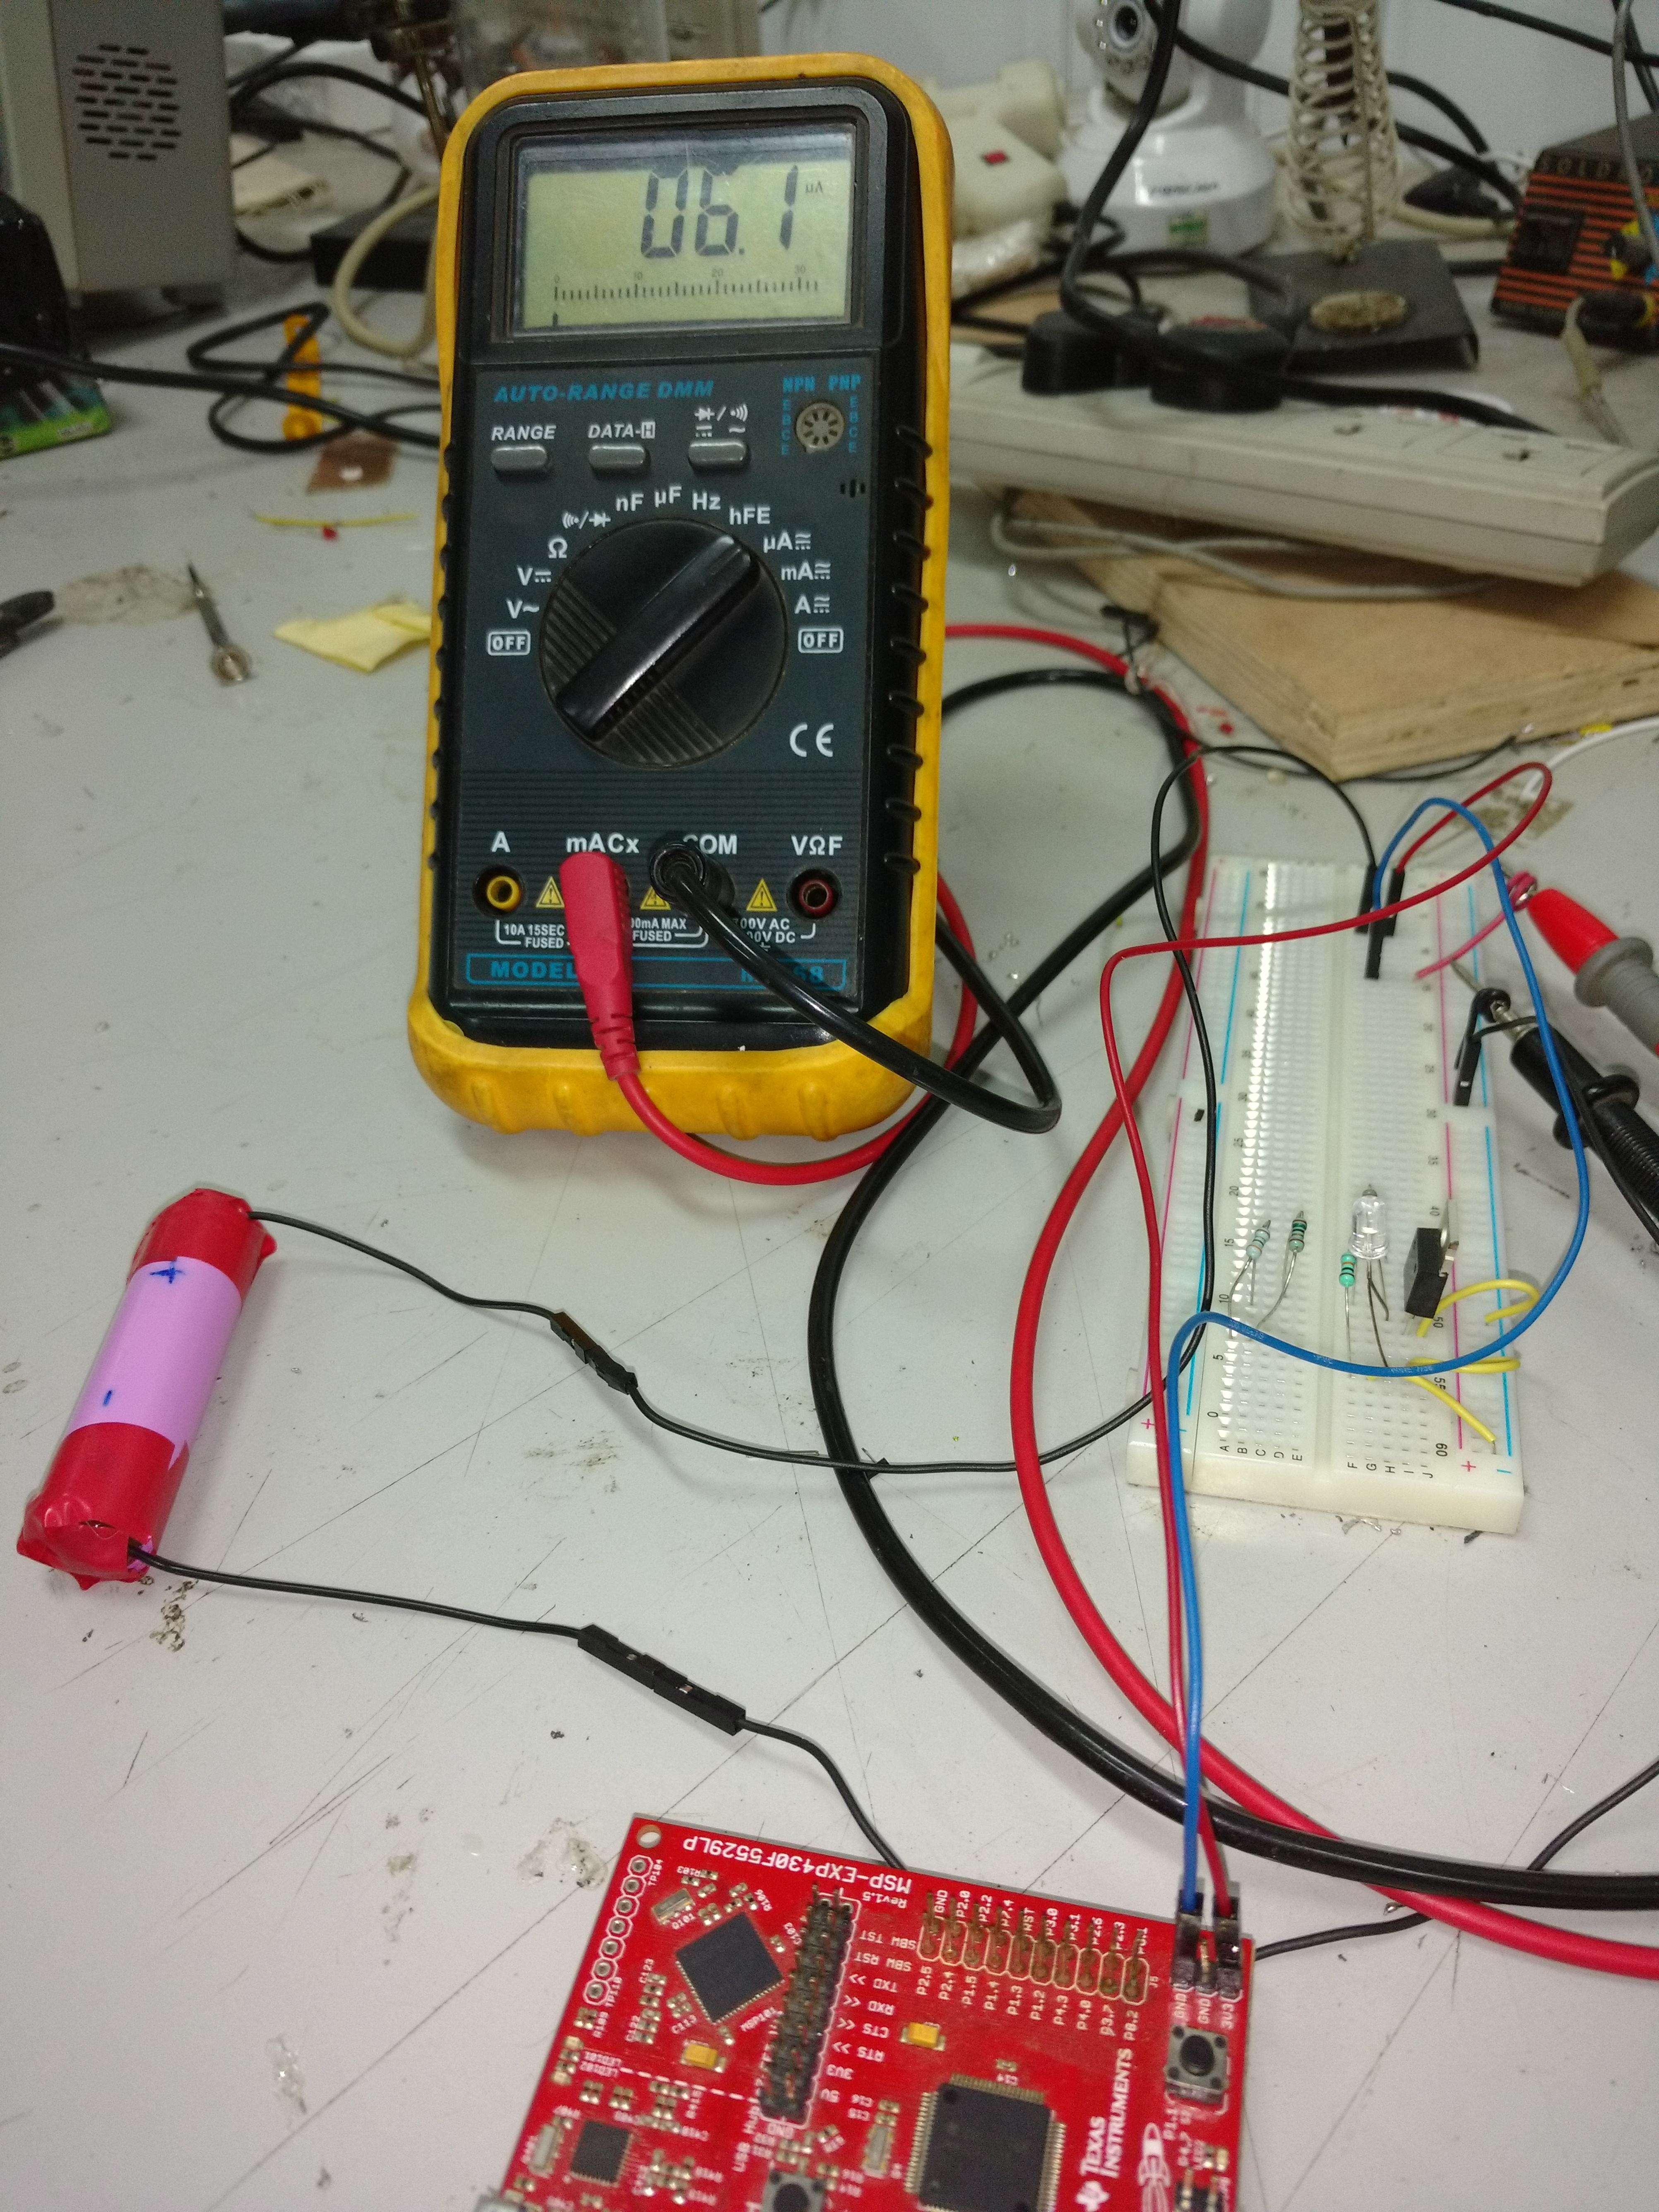
\includegraphics[scale=0.05]{perfect_sleep}
%\caption{LPM3 Sleep}
\label{fig:deep sleep}
\end{figure}
\end{frame}

\begin{frame}{Field Reading}
\begin{figure}[!ht]
	\centering
\includegraphics[scale=0.3]{readings}
%\caption{Sensor Node reading}
\label{fig:SN4_reading}
\end{figure}
\end{frame}

\section{Discussion}
\begin{frame}{Discussion and Challenges}
\begin{itemize}
\item Selecting right Zigbee module \\[0.5cm]
\item Configuring controller to operate in low power mode  \\[0.5cm]
\item Computing average power of system \\[0.5cm]
\item Designing protocol to read value from all sensor node \\[0.5cm]
\item Design of casing for sensor node to withstand outdoor environment \\[0.5cm]
\end{itemize}
\end{frame}

\begin{frame}{Future Work}
\begin{itemize}
\item Interface different sensors and use effective stack design \\[1cm]
\item Trying different topologies, count and location of node for terrace farm\\[1cm]
\item Design of weather proof casing and small form factor sensor node \\[1cm]
\item Simulating the network 
\end{itemize}
\end{frame}

\begin{frame}{References}
\begin{thebibliography}{9}
\bibitem{zigbee_book} Shahin Farahani, "ZigBee Wireless Networks and Transceivers", Book chapters.

\bibitem{dht_22} Aosong Electronics Co.Ltd, DHT22 Datasheet, \url{https://www.sparkfun.com/datasheets/Sensors/Temperature/DHT22.pdf} 

\bibitem{msp430_datasheet} Texas Instruments, "Datasheet for MSP430F552x, MSP430F551x Mixed-Signal Microcontroller" \url{http://www.ti.com/lit/ds/symlink/msp430f5529.pdf}

\bibitem{workshop_guide} Texas Instruments, "MSP430 Design Workshop, Student Guide", Rev.4.01, Feburary,2015
\end{thebibliography}
\end{frame}

\begin{frame}{References}
\begin{thebibliography}{9}
\bibitem{comparative_study}  Jin-Shyan Lee, Yu-Wei Su, and Chung-Chou Shen, "A Comparative Study of Wireless Protocols: Bluetooth, ZigBee, and Wi-Fi", The 33rd Annual Conference of the IEEE Industrial Electronics Society (IECON), Nov. 5-8, 2007, Taiwan

\bibitem{building_WSN} Robert Faludi, "Building Wireless Sensor Networks"

\bibitem{sanam_MTP report} Sanam Shakya, "Sensor Development and Energy Analysis of Low Power Nodes for Wireless Sensor Network", Master of Technology, Dissertation Report, IIT Bombay

\bibitem{WSN_agri} Tamoghna Ojha, Sudip Misra, Narendra Singh Raghuwanshi, "Wireless sensor networks for agriculture: The state-of-the-art in practice and future challenges", Computers and Electronics in Agriculture, September,2015

\end{thebibliography}
\end{frame}

\end{document}


\end{document}